\section{Abstract transport of cells}\label{sec:cells}

\subsection{Region Graver sets and the survival criterion}
\begin{lemma}\label{lem:regionG}
For every lattice $\Lambda\subseteq\Z^k$, $\Gr_q(\Lambda)=\{g\in\Gr(\Lambda):|g_i|\le q_i\ \forall i\}$.
\end{lemma}
\prov{CW-0466}{P2-L1}{PROVED}{FULL}
\begin{proof}
If $h\cm g$ and $|g_i|\le q_i$ then $|h_i|\le q_i$, so every conformal subvector of a vector of the box lies in the box; minimality within the box and within $\Lambda$ coincide for vectors of the box. \qedhere
\end{proof}
\begin{theorem}[generator survival without the target complex]\label{thm:P2T2}
Let $g\in\Gr_q(\Lambda)$. Then $g\in\Gr_q(\Lambda')$ iff $g\in\Lambda'$ and no $v\in\Lambda'\setminus\{0,g\}$ satisfies $v\cm g$. Only $\prod_i(|g_i|+1)-2$ candidate vectors $v$ have to be inspected, and only $\chi_{b'}$ is needed.
\end{theorem}
\prov{CW-0469}{P2-T2}{PROVED}{FULL}
\begin{proof}
Definition of conformal minimality and \cref{lem:regionG}; the candidates are the integer points of the conformal box of $g$. \qedhere
\end{proof}
\begin{theorem}[abstract-cell transport]\label{thm:cell-transport}
Let $\Lambda,\Lambda'$ be lattices, $Q$ a common box, and $c$ a cell of $\Kabs(\Lambda,Q)$. Then
\[
c\in\Kabs(\Lambda',Q)\iff V(c)\subseteq F(\Lambda',Q)\ \text{and}\ \mathrm{Gen}(c)\subseteq\Gr_q(\Lambda').
\]
Put $S=\Gr_q(\Lambda)\cap\Gr_q(\Lambda')$. Then (1) if $\Lambda\subseteq\Lambda'$ all $0$-cells persist, and a $j$-cell $c$ persists iff $\mathrm{Gen}(c)\subseteq S$; (2) no cell of dimension $>\rk\langle S\rangle$ persists; in particular $S=\emptyset$ implies that all cells of positive dimension are lost, and $\rk\langle S\rangle=1$ implies that all $2$-cells are lost; (3) if $\Gr_q(\Lambda)\subseteq\Gr_q(\Lambda')$ and $\Lambda\subseteq\Lambda'$ then $\Kabs(\Lambda,Q)\subseteq\Kabs(\Lambda',Q)$.
\end{theorem}
\prov{CW-0470}{P2-T3}{PROVED}{FULL}
\begin{proof}
($\Rightarrow$) If $c$ is a cell of $\Kabs(\Lambda',Q)$ its vertices are in $F(\Lambda',Q)$ and, by \cref{lem:intrinsic}, $\mathrm{Gen}(c)$ is the set of edge vectors at its smallest vertex (up to sign), which lie in $\Gr_q(\Lambda')$ as generators of a cell of $\Lambda'$. ($\Leftarrow$) Let $m$ be the smallest vertex of $c$. Then $\Pil(m;\mathrm{Gen}(c))$ has independent generators in $\Gr_q(\Lambda')$ and all corners in $V(c)\subseteq F(\Lambda',Q)$, so it is a cell of $\Lambda'$; it has vertex set $V(c)$, hence equals $c$. (1)--(3): for $\Lambda\subseteq\Lambda'$ the vertex condition is automatic; a cell with $j$ independent generators in $S$ needs $j\le\rk\langle S\rangle$; (3) is (1) read for all cells. \qedhere
\end{proof}
This is the general form of the survival rule (ER-15): the earlier statement that a cell survives iff its generators lie in $\Gr\cap\Gr'$ is correct only when its vertices already lie in $F'$, as they do for $\Lambda\subseteq\Lambda'$.

\subsection{Graver sets of \texorpdfstring{$\Z^k$}{Z\^{}k} and of the even-sum lattice}
\begin{proposition}\label{prop:E25}
For $k\ge2$: $\Gr(\Z^k)=\{\pm e_i\}$ and $\Gr(E_k)=\{\pm2e_i\}\cup\{\pm e_i\pm e_j:i<j\}$. The two sets are disjoint.
\end{proposition}
\prov{CW-0460}{E2-5}{PROVED}{FULL}
\begin{proof}
In $\Z^k$ each $e_i$ is minimal, and any nonzero vector dominates some $\pm e_i$. In $E_k$: $e_i\notin E_k$, so $2e_i$ and $e_i\pm e_j$ have no proper nonzero conformal lattice subvector (the only candidates are $\pm e_i,\pm e_j$), hence are minimal. Conversely let $0\ne\lambda\in E_k$. If $|\lambda_i|\ge2$ for some $i$ and $\lambda\ne\pm2e_i$, then $2\,\mathrm{sign}(\lambda_i)e_i\prec\lambda$ is a lattice vector, so $\lambda$ is not minimal. If all $|\lambda_i|\le1$, the support has even size $\ge2$; if it has $\ge4$ elements, then $\mathrm{sign}(\lambda_i)e_i+\mathrm{sign}(\lambda_j)e_j\prec\lambda$ for two support indices. \qedhere
\end{proof}
(The set $\Gr(E_k)$ is the root system $D_k$ together with $\pm2e_i$.)

\subsection{The three-stage orbit}\label{sec:threestage}
\begin{theorem}[three-stage orbit; all $k$, all admissible prime sets]\label{thm:E21}
Let $k\ge2$, $p_1=2<p_2<\dots<p_k$ primes with $p_i\equiv2\pmod 3$, $P=\prod p_i$, $x_0=P^4/3$. Then $L(x_0)=P^2$, $G(x_0)=3$, $x_1=\Cmap(x_0)=2P^4/3$, $x_2=\Cmap(x_1)=P^4$, and
\begin{center}\small
\begin{tabular}{@{}lccc@{}}\toprule
 & $x_0$ & $x_1$ & $x_2$\\\midrule
reduced denominator & $3$ & $3$ & $1$\\
box $q$ & $(2,\dots,2)$ & $(2,\dots,2)$ & $(2,\dots,2)$\\
$|F|$ & $(3^k-1)/2$ & $(3^k-1)/2$ & $3^k-1$\\
relation lattice & $E_k$ & $E_k$ & $\Z^k$\\
$D$ & $D_0$ & $=D_0$ & $\supsetneq D_0$\\\bottomrule
\end{tabular}
\end{center}
\end{theorem}
\prov{CW-0456}{E2-1}{PROVED}{FULL}
\begin{proof}
$d^2\mid P^4\iff d\mid P^2$, so $d=\prod p_i^{\alpha_i}$ with $\alpha\in\{0,1,2\}^k$. Since $p_i\equiv-1\pmod3$, $d\equiv(-1)^{\sum\alpha_i}$; thus $D(x_0)$ corresponds to the nonzero even-weight vectors, $(3^k+1)/2-1=(3^k-1)/2$ of them. The vectors $2e_i$ (that is, $d=p_i^2$) lie in $D(x_0)$ and every $d$ divides $P^2$, so $L=P^2$. Every $d-1$ is divisible by $3$, and $4=2^2\in D(x_0)$ has $d-1=3$, so $G=3$. Hence $\Cmap(x_0)=P^4/3+P^4/3=2P^4/3$. In $x_1$ the numerator $2P^4$ is prime to $3$ and $v_2(2P^4)=5$, $\lfloor5/2\rfloor=2$; the active primes, the box, and (since $d^2\mid2P^4\iff d\mid P^2$) the set $D$ are unchanged, so are $L,G$, and $\Cmap(x_1)=2P^4/3+P^4/3=P^4$. For $x_2=P^4$ the denominator is $1$, $D(x_2)$ is the set of all divisors $\ge2$ of $P^2$ ($3^k-1$ of them) and the lattice is $\Z^k$. \qedhere
\end{proof}
\begin{corollary}[all positive-dimensional cells are lost]\label{cor:threestage}
For the transition $x_1\to x_2$ of \cref{thm:E21} and every $k\ge2$: all vertices persist, no cell of positive dimension of $\Kabs(E_k,Q)$ is a cell of $\Kabs(\Z^k,Q)$, although $D(x_1)\subsetneq D(x_2)$. The transition $x_0\to x_1$ is the identity on $(\Lambda,Q)$.
\end{corollary}
\prov{CW-0461}{E2-6}{PROVED}{FULL}
\begin{proof}
$E_k\subseteq\Z^k$ gives $F\subseteq F'$. By \cref{prop:E25} $S=\Gr(E_k)\cap\Gr(\Z^k)=\emptyset$ (the boxes $[-2,2]^k$ contain all of both Graver sets), so \cref{thm:cell-transport}(2) applies. \qedhere
\end{proof}
The corollary generalises the specimen $P=110$, $k=3$, in which $13\to13\to26$ points; that specimen has the following exact counts, obtained here by independent exact code (\texttt{scripts/run\_exact\_checks.py}).
\begin{proposition}[specimen $k=3$, FINITE-EXACT]\label{prop:specimen}
For $\Lambda=E_3$ and $\Lambda'=\Z^3$ with $Q=[0,2]^3$: the f-vectors of $\Kabs$ are $(13,45,36,3)$ and $(26,51,33,7)$; the Betti numbers over $\Q$ are $(1,6,6,0)$ and $(1,0,0,0)$; of the source cells $0$ edges, $0$ squares, $0$ cubes persist, with $45,36,3$ lost and $51,33,7$ new.
\end{proposition}
\prov{CW-0464}{E2-10}{FINITE-EXACT}{FINITE}
\noindent These are counts for one specimen ($k=3$, box $[0,2]^3$), obtained by exhaustive enumeration, with $\partial\partial=0$ checked. The Betti numbers of the realised union $U$ ($(1,0,18,0)$ for the source and $(1,0,0,0)$ for the target) and the statement that $\Kabs(E_3,Q)$ is not embedded are reported by the release from an exact nerve computation and are cited, not re-derived here; the realised $b_2=18$ differs from the abstract $b_2=6$, which is why every topological statement must name its object.
\begin{figure}[tbp]\centering
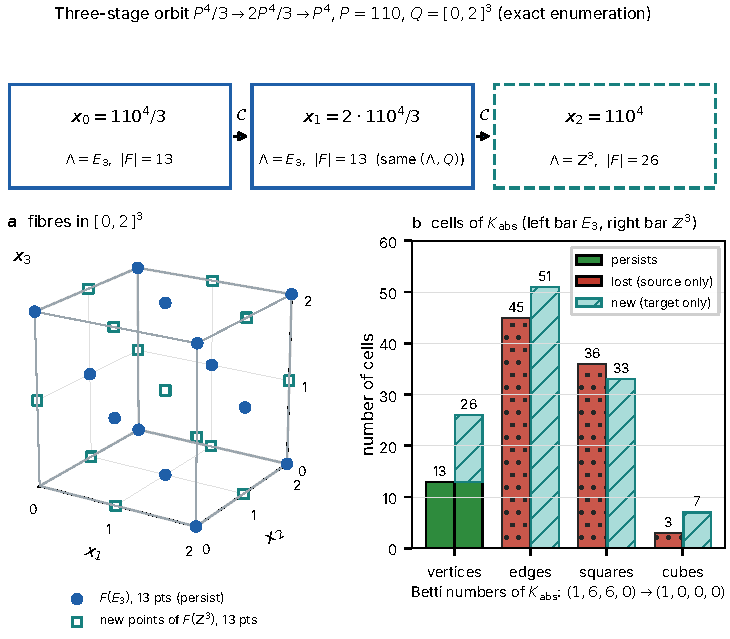
\includegraphics[width=0.78\textwidth]{fig03_three_stage}
\caption{The three-stage orbit $P^4/3\to2P^4/3\to P^4$ for $P=110$, $k=3$, $Q=[0,2]^3$ (\cref{thm:E21,cor:threestage,prop:specimen}; \emph{exact computation}). The first step is the identity on $(\Lambda,Q)=(E_3,Q)$; the second enlarges $E_3$ to $\Z^3$ ($13\to13\to26$ occurrences). (a)~Fibres: the $13$ points of $F(E_3,Q)$ persist, $13$ new points of $F(\Z^3,Q)$ appear. (b)~Cell counts of the abstract complexes $\Kabs(E_3,Q)$, f-vector $(13,45,36,3)$, and $\Kabs(\Z^3,Q)$, f-vector $(26,51,33,7)$: all $13$ vertices persist (green) and no positive-dimensional cell does (red: lost; hatched teal: new). The abstract Betti numbers change from $(1,6,6,0)$ to $(1,0,0,0)$. Only abstract complexes are counted; the realised unions are compared in \cref{sec:realised}.}\label{fig:threestage}
\end{figure}

\subsection{A planar family with exact edge counts}
\begin{theorem}\label{thm:P2TF1}
Let $x_h=21^{2h}/5$, $h\ge1$. (i) $D(x_h)=\{3^a7^b:a\equiv b\ (4),\ 0\le a,b\le h,\ (a,b)\ne0\}$, $L=21^h$, $G=20$, $\Cmap(x_h)=x_h'=21^{2h}/4$; the primes $(3,7)$ and the box $(h,h)$ are unchanged. (ii) $\Lambda=\{a\equiv b\ (4)\}\subsetneq\Lambda'=\{a\equiv b\ (2)\}$. (iii) $\Gr(\Lambda)=\pm\{(1,1),(4,0),(0,4),(1,-3),(3,-1),(2,-2)\}$, $\Gr(\Lambda')=\pm\{(1,1),(1,-1),(2,0),(0,2)\}$, and $\Gr_h(\Lambda)\cap\Gr_h(\Lambda')=\{\pm(1,1)\}$ for every $h\ge1$. (iv) All vertices persist; the persisting edges are exactly the edges $\{u,u+(1,1)\}$; no $2$-cell persists; their number is
\[
E_{\mathrm{kept}}(h)=\sum_{r=0}^3c_r(h)^2-1,\qquad c_r(h)=\#\{n\in[0,h-1]:n\equiv r\ (4)\}.
\]
\end{theorem}
\prov{CW-0471}{P2-TF1}{PROVED}{FULL}
\begin{proof}
(i) $d^2\mid21^{2h}$ iff $d\mid21^h$, $d=3^a7^b$. Modulo $5$: $7\equiv2\equiv3^3$ and $3$ has order $4$, so $3^a7^b\equiv3^{a+3b}\equiv3^{a-b}$, which is $1$ iff $a\equiv b\ (4)$. Then $(h,h)\in D$, so $L=21^h$. Every such $d$ has $a+b$ even; since $3\equiv7\equiv-1\pmod4$ we get $d\equiv1\pmod4$, with $5\mid d-1$: $20\mid G$. And $21\in D$ ($a=b=1$) has $21-1=20$, so $G=20$. Therefore $\Cmap(x_h)=21^{2h}(\tfrac15+\tfrac1{20})=21^{2h}/4$; the numerator is unchanged, so primes and box are unchanged. (ii) Modulo $4$: $3^a7^b\equiv(-1)^{a+b}$; modulo $5$ as in (i). (iii) Let $v=(a,b)\ne0$ in $\Lambda$. If $a,b\ge1$ then $(1,1)\cm v$; if $b=0$ then $4\mid a$ and $(4,0)\cm v$; likewise $a=0$. If $a>0>b$ put $c=-b>0$, so $a+c\equiv0\ (4)$; $a\ge4$ gives $(4,0)\cm v$ and $c\ge4$ gives $(0,-4)\cm v$, so minimal vectors have $a,c\le3$ and $a+c=4$: $(1,-3),(2,-2),(3,-1)$, each minimal because every nonzero proper conformal subvector has $a'+c'\in\{1,2,3\}$. For $\Lambda'$: this is $\Gr(E_2)$ by \cref{prop:E25}. The source vectors $(4,0),(0,4),(1,-3),(3,-1),(2,-2)$ dominate $(2,0),(0,2),(1,-1),(1,-1),(1,-1)$ respectively, all in $\Lambda'$, so they are not target Graver vectors; $(1,1)$ is common; the target vectors $(1,-1),(2,0),(0,2)$ are not in $\Lambda$. Region sets are the intersections with $[-h,h]^2$ (\cref{lem:regionG}); $(1,1)$ lies in the box for $h\ge1$. (iv) $\Lambda\subseteq\Lambda'$ gives $F\subseteq F'$. By \cref{thm:cell-transport} an edge persists iff its generator is in $S=\{\pm(1,1)\}$, and a $2$-cell needs two independent generators in $S$: impossible. The $(1,1)$-edges are $\{u,u+(1,1)\}$ with $u=(a,b)$, $a\equiv b\ (4)$, $0\le a,b\le h-1$, $u\ne0$; counting residue classes gives $\sum c_r^2-1$. \qedhere
\end{proof}
\begin{remark}
The release also gives closed quasi-polynomial formulas for the number of source and target edges and the limiting survival ratio $1/6$; the quasi-polynomials for the source and target edge counts are valid only for $h\ge4$ (ER-17), whereas $E_{\mathrm{kept}}(h)$ above holds for all $h\ge1$. Those counting formulas are not reproduced here. For $h=1,\dots,12$ the value $E_{\mathrm{kept}}$, the equality $S=\{\pm(1,1)\}$ and the non-persistence of $2$-cells were confirmed by direct exact enumeration (\texttt{scripts/run\_exact\_checks.py}); this confirms the proof and is not a substitute for it. \Cref{fig:planar} shows $h=8$.
\end{remark}
\begin{figure}[tbp]\centering
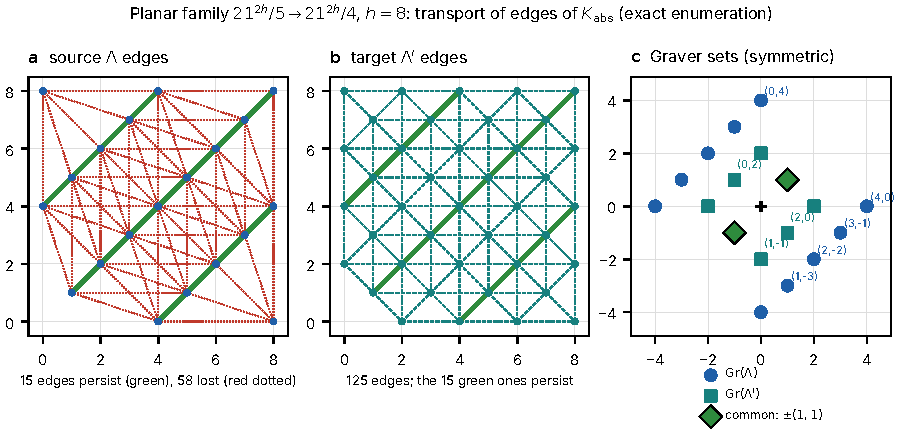
\includegraphics[width=0.98\textwidth]{fig04_planar_edges}
\caption{Planar family $21^{2h}/5\to21^{2h}/4$ for $h=8$ (\cref{thm:P2TF1}; \emph{exact computation} of $\Kabs$). (a)~The $73$ edges of $\Kabs(\Lambda,Q)$, $\Lambda=\{a\equiv b\ (4)\}$: the $15=E_{\mathrm{kept}}(8)$ edges with generator $\pm(1,1)$ persist (green, thick) and the other $58$ are lost (red, dotted). (b)~The $125$ edges of $\Kabs(\Lambda',Q)$, $\Lambda'=\{a\equiv b\ (2)\}$, with the persisting edges again green. (c)~The Graver sets $\Gr(\Lambda)$ and $\Gr(\Lambda')$ (each symmetric under $v\mapsto-v$) in the window $[-4,4]^2$; they share only $\pm(1,1)$, which is why only $(1,1)$-edges can persist (\cref{thm:cell-transport}). The panels show abstract complexes (edges only), not the realised unions.}\label{fig:planar}
\end{figure}
